\newpage
\subsection{Caso d'uso UC13: Ricerca utente}
\label{UC13}
\begin{figure}[ht]
	\centering
	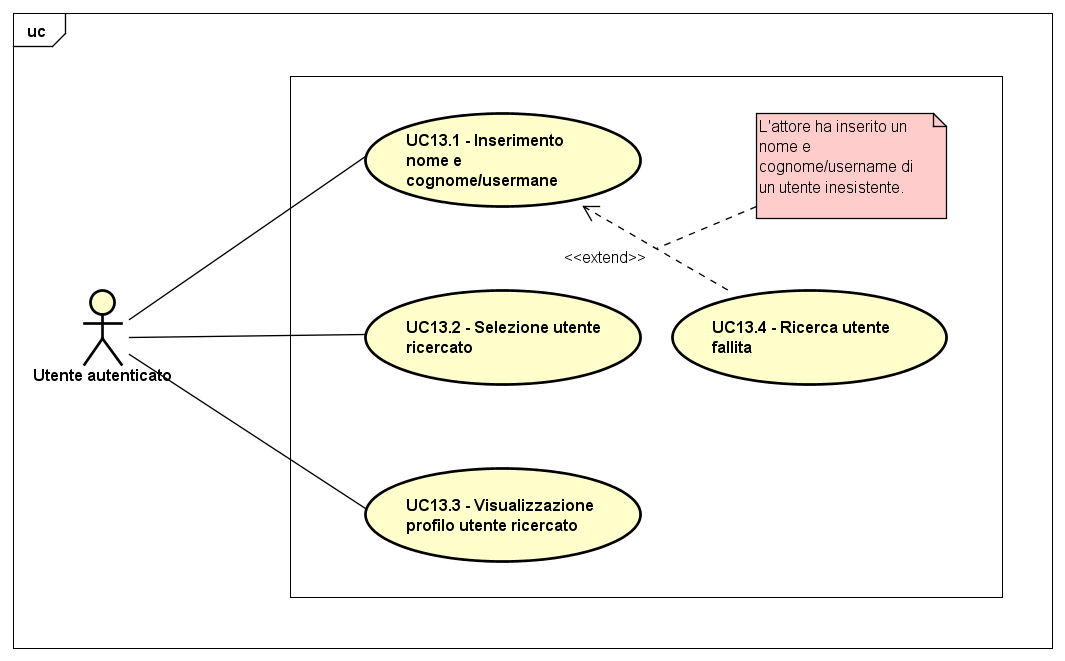
\includegraphics[scale=0.5]{UML/UC13.png}
	\caption{UC13: Ricerca utente}
\end{figure}
\FloatBarrier
\begin{itemize}
	\item \textbf{Attori}: utente autenticato, utente autenticato pro;
	\item \textbf{Descrizione}: l'attore può ricercare un utente registrato al sistema;
	\item \textbf{Precondizione}: il sistema visualizza la barra per la ricerca degli utenti;
	\item \textbf{Postcondizione}: il sistema visualizza il profilo dell'utente ricercato;
	\item \textbf{Scenario principale}:
	\begin{enumerate}
		\item L'attore può inserire nome e cognome/username dell'utente che vuole ricercare (UC13.1);
		\item L'attore può selezionare l'utente ricercato per visualizzarne il profilo (UC13.2).
	\end{enumerate} 
	\item \textbf{Estensioni}: la ricerca dell'utente è fallita (UC13.3);
\end{itemize}

\subsubsection{Caso d'uso UC13.1: Inserimento nome e cognome/usermane}

\begin{itemize}
	\item \textbf{Attori}: utente autenticato, utente autenticato pro;
	\item \textbf{Descrizione}: l'attore può inserire nome e cognome/username di un utente nella barra di ricerca;
	\item \textbf{Precondizione}: il sistema visualizza la barra per la ricerca degli utenti;
	\item \textbf{Postcondizione}: l'attore ha inserito nome e cognome/username dell'utente che vuole ricercare;
	\item \textbf{Scenario principale}: l'attore inserisce il nome e cognome/username dell'utente che vuole ricercare.
\end{itemize}

\subsubsection{Caso d'uso UC13.2: Selezione utente ricercato}

\begin{itemize}
	\item \textbf{Attori}: utente autenticato, utente autenticato pro;
	\item \textbf{Descrizione}: l'attore può selezionare l'utente ricercato per visualizzarne il profilo;
	\item \textbf{Precondizione}: il sistema visualizza la pagina con l'elenco dei risultati della ricerca utente;
	\item \textbf{Postcondizione}: il sistema visualizza il profilo dell'utente selezionato;
	\item \textbf{Scenario principale}: l'attore seleziona l'utente ricercato per visualizzarne il profilo.
\end{itemize}

\subsubsection{Caso d'uso UC13.3: Visualizzazione profilo utente ricercato}
\label{UC13.3}
\begin{figure}[h]
	\centering
	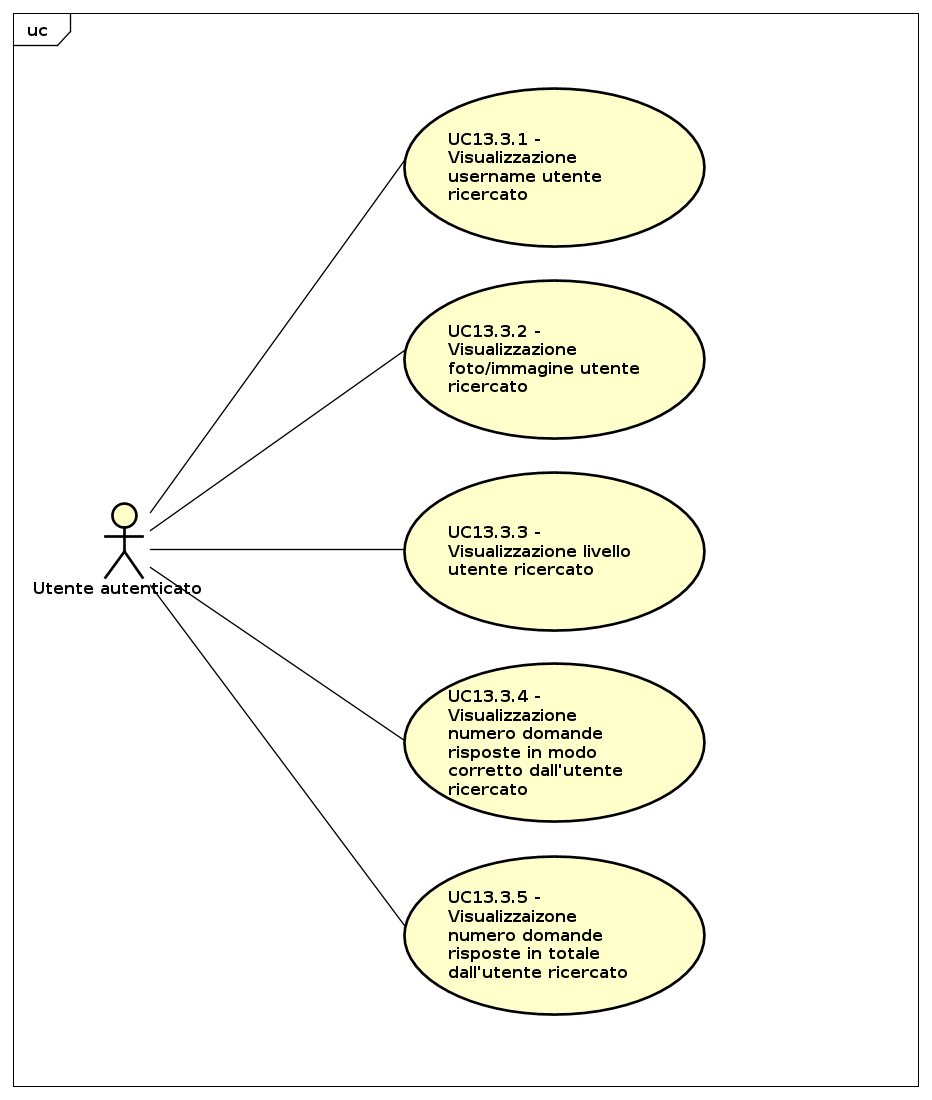
\includegraphics[scale=0.5]{UML/UC13_3.png}
	\caption{UC13.3: Visualizzazione profilo utente ricercato}
\end{figure}
\FloatBarrier
\begin{itemize}
	\item \textbf{Attori}: utente autenticato, utente autenticato pro;
	\item \textbf{Descrizione}: l'attore può visualizzare il profilo utente ricercato;
	\item \textbf{Precondizione}: il sistema visualizza il profilo dell'utente selezionato dopo la ricerca;
	\item \textbf{Postcondizione}: l'attore visualizza il profilo utente ricercato;
	\item \textbf{Scenario principale}:
	\begin{enumerate}
		\item L'attore può visualizzare l'username dell'utente ricercato (UC13.3.1);
		\item L'attore può visualizzare la foto/immagine dell'utente ricercato (UC13.3.2);
		\item L'attore può visualizzare il livello dell'utente ricercato (UC13.3.3);
		\item L'attore può visualizzare il numero delle domande risposte in modo corretto dall'utente ricercato (UC13.3.4);
		\item L'attore può visualizzare il numero delle domande risposte in totale dall'utente ricercato (UC13.3.5).
	\end{enumerate}
\end{itemize}

\subsubsection{Caso d'uso UC13.3.1: Visualizzazione username utente ricercato}
\begin{itemize}
	\item\textbf{Attori}: utente autenticato, utente autenticato pro;
	\item\textbf{Descrizione}: l'attore può visualizzare l'username dell'utente ricercato;
	\item\textbf{Precondizione}: il sistema visualizza la pagina utente ricercato;
	\item\textbf{Postcondizione}: l'attore visualizza l'username dell'utente ricercato;
	\item\textbf{Scenario principale}: l'attore visualizza l'username dell'utente ricercato.
\end{itemize}

\subsubsection{Caso d'uso UC13.3.2: Visualizzazione foto/immagine utente ricercato}
\begin{itemize}
	\item\textbf{Attori}: utente autenticato, utente autenticato pro;
	\item\textbf{Descrizione}: l'attore può visualizzare la foto/immagine dell'utente ricercato;
	\item\textbf{Precondizione}: il sistema visualizza la pagina utente ricercato;
	\item\textbf{Postcondizione}: l'attore visualizza la foto/immagine dell'utente ricercato;
	\item\textbf{Scenario principale}: l'attore visualizza la foto/immagine dell'utente ricercato.
\end{itemize}

\subsubsection{Caso d'uso UC13.3.3: Visualizzazione livello utente ricercato}
\begin{itemize}
	\item\textbf{Attori}: utente autenticato, utente autenticato pro;
	\item\textbf{Descrizione}: l'attore può visualizzare il livello dell'utente ricercato;
	\item\textbf{Precondizione}: il sistema visualizza la pagina utente ricercato;
	\item\textbf{Postcondizione}: l'attore visualizza il livello dell'utente ricercato;
	\item\textbf{Scenario principale}: l'attore visualizza il livello dell'utente ricercato.
\end{itemize}

\subsubsection{Caso d'uso UC13.3.4: Visualizzazione numero domande risposte in modo corretto dall'utente ricercato}
\begin{itemize}
	\item\textbf{Attori}: utente autenticato, utente autenticato pro;
	\item\textbf{Descrizione}: l'attore può visualizzare il numero di domande risposte in modo corretto dall'utente ricercato;
	\item\textbf{Precondizione}: il sistema visualizza la pagina dell'utente ricercato;
	\item\textbf{Postcondizione}: l'attore visualizza il numero di domande risposte in modo corretto dall'utente ricercato;
	\item\textbf{Scenario principale}: l'attore visualizza il numero di domande risposte in modo corretto dall'utente ricercato.
\end{itemize}

\subsubsection{Caso d'uso UC13.3.5: Visualizzazione numero domande risposte in totale dall'utente ricercato}
\begin{itemize}
	\item\textbf{Attori}: utente autenticato, utente autenticato pro;
	\item\textbf{Descrizione}: l'attore può visualizzare il numero di domande risposte in totale;
	\item\textbf{Precondizione}: il sistema visualizza la pagina dell'utente ricercato;
	\item\textbf{Postcondizione}: il sistema visualizza il numero di domande risposte in totale dall'utente ricercato;
	\item\textbf{Scenario principale}: il sistema visualizza il numero di domande risposte in totale dall'utente ricercato.
\end{itemize}

\subsubsection{Caso d'uso UC13.4: Ricerca utente fallita}

\begin{itemize}
	\item \textbf{Attori}: utente autenticato, utente autenticato pro;
	\item \textbf{Descrizione}: l'attore può visualizzare un messaggio d'errore nel caso si fosse verificato lo scenario alternativo durante la fase di ricerca dell'utente;
	\item \textbf{Precondizione}: il sistema ha ricevuto un nome e cognome/username vuoto o non valido;
	\item \textbf{Postcondizione}: il sistema avvisa l'attore dell'errore verificatosi tramite un opportuno messaggio;
\item\textbf{Scenario principale}: l'attore visualizza un messaggio d'errore.
\end{itemize}